%%%%%%%%%%%%%%%%%%%%%%%%%%%%%%%%%%%%%%%%%%%%%%%%%%%%%%%%%%%%%%%%%%%%%%%%
%%%%%%%%%%%%%%%%%%%%%%%%%%%%%%%%%%%%%%%%%%%%%%%%%%%%%%%%%%%%%%%%%%%%%%%%
\begin{frame}
  \frametitle{Plan}

  \begin{itemize}
  \item 8 avril 2021 : \myhref{https://www.canal-u.tv/video/groupe_calcul/pourquoi_julia.60773}{Café Calcul - Pourquoi Julia ?}
  \item le problème des deux languages (script + bas niveau) $\Rightarrow$ \textcolor{violet}{\bf Julia}
  \item le problème des deux (en fait plus) modèles de programmation (en mémoire partagée) $\Rightarrow$ Portabilité de performance
  \end{itemize}

  \begin{center}
    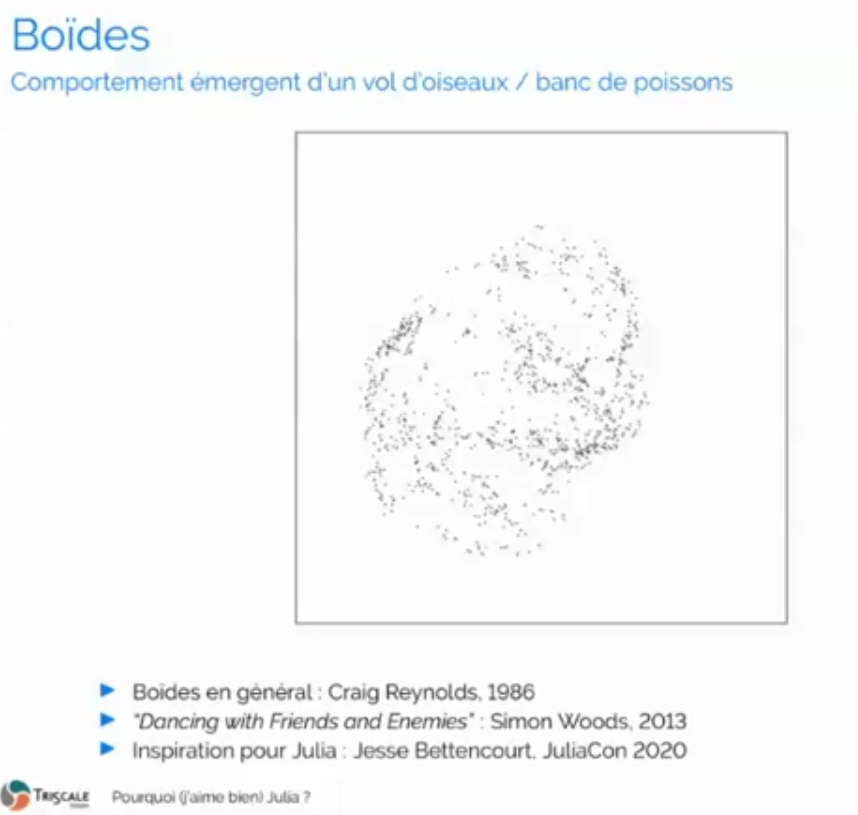
\includegraphics[width=4cm]{julia/pourquoi_julia1}
    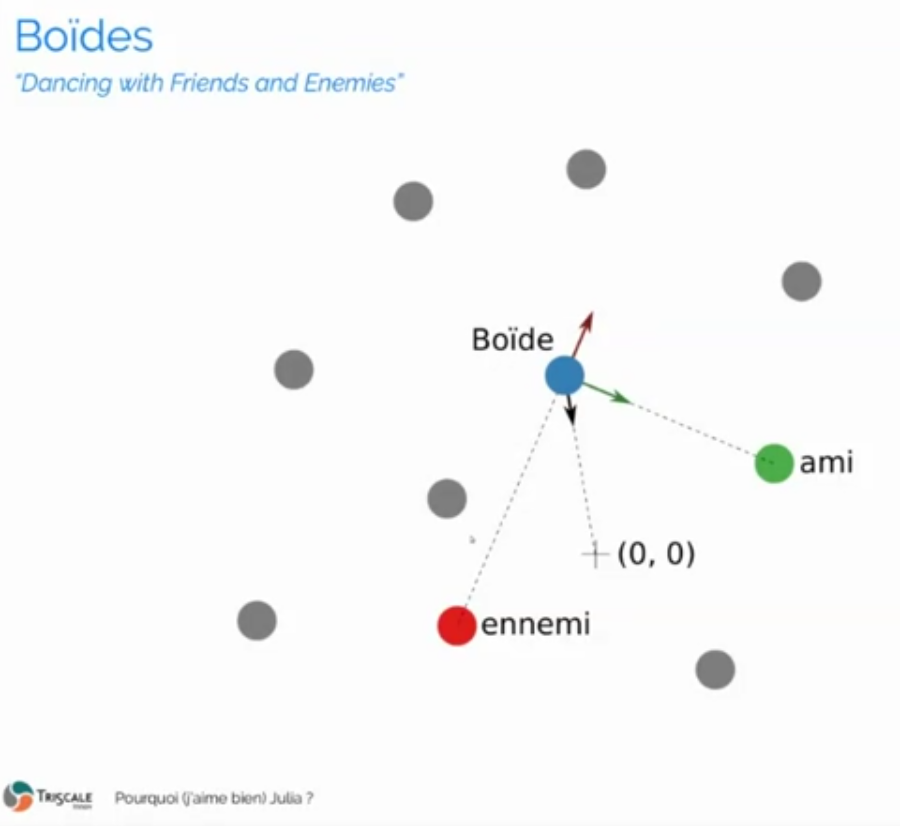
\includegraphics[width=4cm]{julia/pourquoi_julia2}
  \end{center}

\end{frame}
